\shorthandoff{:!} %règle un problème de compatibilité avec babel
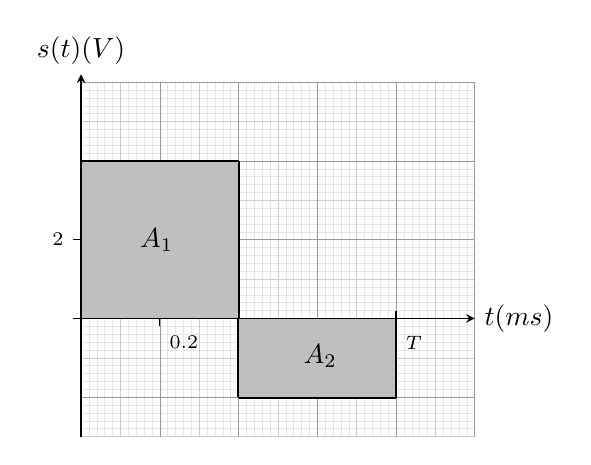
\begin{tikzpicture}[scale=1]
	%papier milli
	\draw [very thin, gray!20] (0,-1.5) grid[step=0.1] (5,3);
	\draw [very thin, black!20] (0,-1.5) grid[step=0.5] (5,3);
	\draw [very thin, black!40] (0,-1.5) grid[step=1] (5,3);
	%fin 
	%axes
	\draw[->,>=stealth] (-0.1,0) -- (5,0) node[right] {$t (ms)$};
	%stealth définit un style de flèche, "furtif"
	\draw[->,>=stealth] (0,-1.5) -- (0,3.1)node[above] {$s(t) (V)$};;
	\draw (1,0.1) -- (1,-0.1) node [below right] {{\scriptsize $0.2$}}; %échelle abscisse
	\draw (0.1,1) -- (-0.1,1) node [left] {{\scriptsize $2$}}; %échelle ordonnée
	%fin
	%lLe signal
	\draw [color=black,line width=1pt, smooth] (0,2) -- (2,2);
	\draw [color=black,line width=1pt, smooth] (2,-1) -- (4,-1);
	\draw [color=black,line width=1pt, smooth] (0,-1) -- (0,2);
	\draw [color=black,line width=1pt, smooth] (2,-1) -- (2,2);
	%\draw (0.1,2) -- (-0.1,2) node [left] {{\scriptsize $S_0$}}; 
	\draw (4,0.1) -- (4,-0.1) node [below right] {{\scriptsize $T$}}; 
	%  Tracer de l'aire sous la courbe
	\draw[fill=lightgray] (0,0) -- (0,2) -- (2,2) -- (2,0) node[midway,left=20pt]{$A_1$}--cycle;
	\draw[fill=lightgray] (2,0) -- (4,0) -- (4,-1) -- (2,-1) node[above=15pt,right=20pt]{$A_2$}--cycle;
\end{tikzpicture} 
\shorthandon{:!}

